% FedCLEAR, PAKDD submission (LNCS). Version 2: calibrated repair with a referee gate (CLEAR-v2).
%
\documentclass[runningheads]{llncs}
%
\usepackage[T1]{fontenc}
\usepackage{newtxtext}
\usepackage[varvw]{newtxmath}
\usepackage{graphicx}
\usepackage{booktabs}
\usepackage{multirow}
\usepackage{float}
\usepackage{algorithm}
\usepackage{algpseudocode}
\algrenewcommand\alglinenumber[1]{\scriptsize #1:}
\usepackage{placeins}   % \FloatBarrier: keep each section's floats inside it
\raggedbottom           % no stretched gaps around the [H] tables
\begin{document}
%
\title{FedCLEAR: Robust Few-Shot Federated Vision-Language Models under Label Noise}

% \author{Quang-Anh Nguyen\inst{1}\orcidID{0000-1111-2222-3333} \and
% Thanh-Hai Tran\inst{1}\orcidID{1111-2222-3333-4444}}
% \authorrunning{Quang-Anh Nguyen et al.}
% \institute{School of Electrical and Electronic Engineering \\
% Hanoi University of Science and Technology, Hanoi, Vietnam \\
% \email{hai.tranthithanh1@hust.edu.vn}}
\maketitle

\begin{abstract}
Federated Prompt Learning (FPL) tunes a short prompt of a frozen vision-language model such as CLIP
across decentralized clients and exchanges only a few thousand parameters per round, which suits
clients with a handful of labelled images. This setting is fragile: when three of ten clients have
noisy labels, the prompt learned by PromptFL on Oxford Pets becomes less accurate than zero-shot CLIP. We propose FedCLEAR (\textbf{Fed}erated \textbf{C}orrupted-\textbf{L}abel
\textbf{E}nhanced \textbf{A}daptive \textbf{R}ecovery), which repairs noisy labels on each client
before local training. Each client compares its labels with a reference prediction that averages the
received global prompt and zero-shot CLIP; the mean excess loss of its labels under this reference decides whether the client needs repair, and its suspect samples are relabelled when the reference is confident and set aside
otherwise. Because the global prompt absorbs wrong labels when noise is heavy, the server calibrates
the reference with a temperature fitted under an explicit label-noise model, and switches this
calibrated repair on only when the clients' early reports show that the reference is reliable.
The extra communication is at most 25 numbers per client and round. On five
datasets with 8 labelled images per class and ten non-IID clients, from three noisy clients up to
75\% noise on every client, FedCLEAR has the best or tied-best average accuracy in nine of the ten
combinations of dataset and scenario, against baselines that include the recent FedRG; with 75\%
pairwise noise on every client it keeps 84.7\% on Pets, where PromptFL falls to 28.8\% and the best
baseline reaches 75.4\%. More labelled images do not remove the problem: with every client noisy,
FedCLEAR stays 12 to 31 points ahead of PromptFL on Pets, Caltech101 and DTD from 8 up to 32 or 64
images per class. Code will be released upon acceptance.

\keywords{Federated learning \and Label noise \and Prompt learning \and Few-shot learning.}
\end{abstract}

\section{Introduction}
The convergence of Federated Learning (FL) \cite{mcmahan2017communication} and large Vision-Language
Models (VLMs) such as CLIP \cite{radford2021learning} has led to Federated Prompt Learning (FPL)
\cite{guo2023promptfl}. Instead of training a full backbone, FPL keeps the VLM frozen on every client
and learns a short continuous prompt collaboratively. Only the prompt, a few thousand parameters,
travels between the clients and the server, which cuts the communication by orders of magnitude and
lets data-scarce clients adapt quickly. This makes FPL a natural choice for federated few-shot
learning, where each participant holds only a few labelled images per class \cite{zhou2022learning}.

A weakness of current FPL methods is that they assume clean local labels. In real deployments, labels
on edge devices come from non-expert tagging, weak automatic labelling or sensor errors, and are often
wrong \cite{tsouvalas2022federated}. In the few-shot regime every image counts, so even a small share of
wrong labels changes the local data substantially.

% To measure this vulnerability, we train four methods in two representative groups: 
% PromptFL (FedAvg with a CoOp prompt) does not correct labels,  FedCorr \cite{xu2022fedcorr}, FedRG \cite{wen2026fedrg} and NLPrompt \cite{pan2025nlprompt} (an FPL) tried to deal with noisy labels, on Oxford Pets and Caltech101 with 8 labelled
% images per class and ten non-IID clients (296 and 800 training images in the whole federation; the
% setup is detailed in Sec.~\ref{sec:exp}). We increase the noise from three noisy clients to every
% client with 50\% and 75\% of noisy labels using the symmetric noisy strategy (Fig.~\ref{fig:fl_noise_impact}).

% [Fig. 1 redrawn 2026-11-16 with the grouping above: PromptFL alone, NLPrompt/FedCorr/FedRG together.
%  Ready to use: uncomment together with the paragraph above if it goes back into the paper.]
% \begin{figure}[H]
%     \centering
%     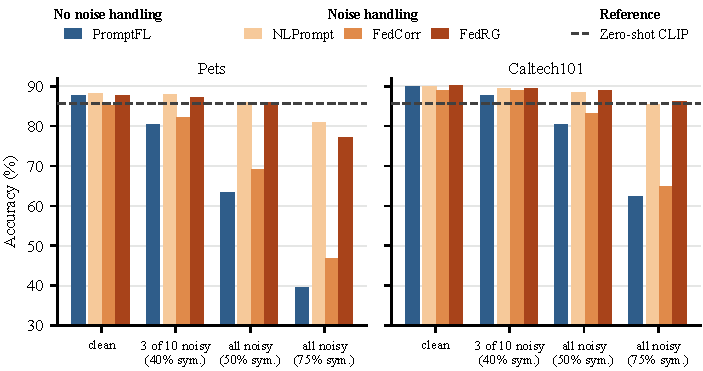
\includegraphics[width=0.9\linewidth]{Figs/NoiseImpact.pdf}
%     \caption{\textbf{Effect of label noise on federated prompt learning} with 8 labelled images per
%     class and 10 non-IID clients (mean of the last 10 rounds over 5 seeds). Blue: PromptFL, which has
%     no noise handling; orange: methods designed for noisy labels. The dashed line is zero-shot CLIP,
%     which uses no training label.}
%     \label{fig:fl_noise_impact}
% \end{figure}



% When no noise-awareness mechanism is employed (PromptFL \cite{guo2023promptfl}), label noise rapidly degrades federated learning performance. With only three out of ten clients exhibiting noisy labels, PromptFL already underperforms zero-shot CLIP on Oxford Pets. When all clients have 75\% label noise, its accuracy drops by 48 percentage points on Oxford Pets and 28 percentage points on Caltech101. 
% % FedCorr and FedRG. While FedCorr \cite{xu2022fedcorr}identifies noisy labels by modeling loss-value distributions with Gaussian Mixture Models (GMMs), FedRG \cite{tian2026fedgr} assesses data cleanliness based on representation geometry. Both methods therefore exhibit greater robustness to label noise than the naive PromptFL baseline. NLPrompt \cite{pan2025nlprompt} further addresses label noise by detecting prediction disagreements between zero-shot semantic anchors and prompt-based predictions, followed by budgeted pseudo-relabeling. Consequently, NLPrompt also demonstrates strong resilience to label noise as well. However, when all clients are affected by label noise, all these methods still underperform zero-shot CLIP on conventional classes. 

These observations reveal a catastrophic failure mode: back-propagating corrupted local
gradients into the shared soft prompt induces severe negative transfer and semantic distortion, a
phenomenon we define as \textbf{Prompt Drift}. In this regime, federated prompt learning is not merely
sub-optimal; it actively harms performance compared to deploying an off-the-shelf zero-shot foundation
model. Mitigating label noise in federated few-shot prompt tuning presents unique challenges that
existing robust FL algorithms fail to address. Conventional noise-tolerant FL frameworks (e.g.,
FedCorr \cite{xu2022fedcorr} and FedLN \cite{tsouvalas2022federated}) rely heavily on statistical noise
estimation techniques, such as fitting Gaussian Mixture Models on the local intrinsic dimension or
the loss distribution, or clustering local feature embeddings; the recent FedRG \cite{wen2026fedrg}
likewise relies on the geometry of the local features. However, under extreme sample scarcity
(few-shot settings), these statistical noise estimators become unreliable due to insufficient sample
density, and none of these methods stays above zero-shot CLIP under heavy noise.
% (Fig.~\ref{fig:fl_noise_impact}).

To bridge this gap, we propose a simple but robust framework named \textbf{FedCLEAR}
(\textit{Federated Corrupted-Label Enhanced Adaptive Recovery}), which leverages the intrinsic
zero-shot semantic capabilities of frozen vision-language models for on-device noise detection and
correction. Recognizing that the frozen CLIP backbone possesses rich prior knowledge independently
of noisy local annotations, FedCLEAR uses zero-shot textual prompts as a reliable ``semantic anchor''
to evaluate local sample credibility. Specifically, our approach consists of two complementary
modules (Fig.~\ref{fig:FEDCLEAR}): (1) a \textit{Noise Detection} module that combines the received global prompt with the
zero-shot anchor into a reference prediction and takes the excess loss of the local labels under this
reference as the metric of noisiness. Based on this metric, it detects the noisy clients and, within
them, the suspect samples. (2) a \textit{Sample Relabeling} module that relabels a suspect sample with
the reference prediction when the reference is confident and sets it aside for the round otherwise.
Under heavy noise, a noise-aware temperature calibrates the reference, a step that the server switches
on only after the clients' first reports show that the reference is reliable. The primary
contributions of this paper are summarized as follows:
\begin{itemize}
    
\item In the initial training rounds, we propose a novel score to assess client and label cleanliness by equally leveraging predictions from the current prompt model and zero-shot CLIP, exploiting the complementary strengths of both.

\item As training progresses and the prompt model becomes more reliable, we introduce an adaptive scoring mechanism that dynamically adjusts the relative trust in the current model and zero-shot CLIP, enabling more reliable identification and correction of noisy labels through pseudo-relabeling.

\item The proposed FedCLEAR maintains the lightweight communication protocol of standard PromptFL, introducing less than 1\% additional communication overhead but achieves the best or tied-best average accuracy in nine out of ten dataset--scenario combinations against state-of-the-art baselines, including the recent FedRG.

\item Extensive experiments on five benchmark datasets (Oxford Pets, Caltech101, DTD, MNIST, and EuroSAT), covering four noise models, noise rates ranging from 25\% to 75\%, and two noise scenarios across non-IID clients. The performance gains are particularly pronounced under heavy label noise.

\end{itemize}

\section{Related works}
\subsection{Federated Prompt Learning}
Unlike standard FL \cite{mcmahan2017communication} that transmits full models, Federated Prompt Learning freezes a vision-language backbone and learns only lightweight prompts. PromptFL \cite{guo2023promptfl} combines CoOp \cite{zhou2022learning} with FedAvg to reduce communication costs. Subsequent works address data heterogeneity via personalized prompts using optimal transport (FedOTP \cite{li2024fedotp}), variable-length prompts (FedPHA \cite{liu2025fedpha}), pre-LayerNorm tuning (NormFit \cite{motamedi2025normfit}), or multi-label extensions (FedMPT \cite{wang2026fedmpt}). However, all these methods assume clean labels, suffering from \textit{Prompt Drift} under label noise. Closest to our work, NLPrompt \cite{pan2025nlprompt} handles noisy labels in centralized prompt tuning via mean-absolute-error loss and optimal transport, which we adapt to FL via FedAvg as a baseline.

\subsection{Learning with Noisy Labels in Federated Learning}
Client-specific label noise exacerbates model drift in FL. Existing defenses typically estimate noise statistics from local training dynamics or feature distributions: FedCorr \cite{xu2022fedcorr} uses local intrinsic dimensionality and Gaussian mixture models (GMMs) across three sequential stages; FedDiv \cite{lijichang2024feddiv} aggregates local loss GMMs; FedGR \cite{tian2026fedgr} exploits slow global memorization; and FedEFC \cite{wacv2025fedefc} combines early stopping with loss correction. Other approaches leverage pretrained or self-supervised representations, including FedLN \cite{tsouvalas2022federated}, FedRG \cite{wen2026fedrg} (von Mises--Fisher mixtures), and FedLTF \cite{zhan2025fedltf} (linear-probe teachers). Because these methods rely on local sample statistics or model training, they become unreliable in few-shot regimes. In contrast, FedCLEAR anchors its noise detection on noise-immune zero-shot CLIP combined with the global prompt.

\section{Proposed method}
\subsection{Preliminary: Federated Prompt Learning}
\begin{figure}[H]
    \centering
    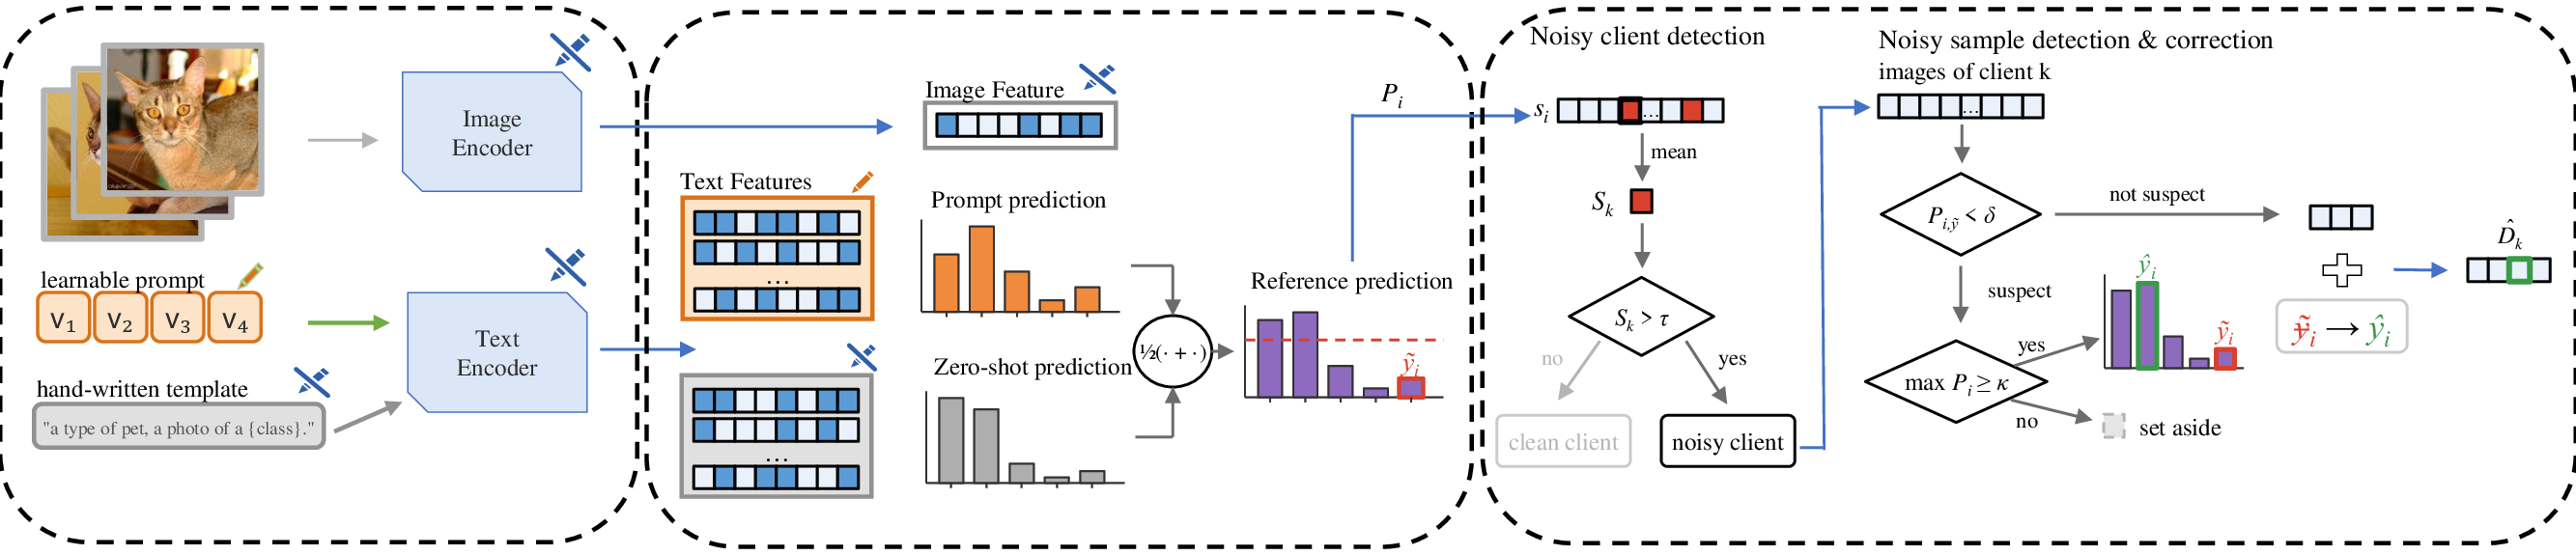
\includegraphics[width=\linewidth]{Figs/Framework.png}
    \caption{\textbf{Overview of FedCLEAR on client $k$ in round $t$.} Left: the frozen CLIP encoders
    give the image feature and the text features of the received global prompt $\mathbf{v}^{t}$ and of
    the hand-written template $\mathbf{t}^{\mathrm{zs}}$. Middle: the prompt prediction and the
    zero-shot prediction are averaged into the reference prediction $\mathbf{P}_i$
    (Eq.~\eqref{eq:ref}); an observed label $\tilde{y}_i$ whose probability falls below the dashed
    level has a positive excess loss $s_i$ (Eq.~\eqref{eq:excess}, look-alike classes ignored).
    Right: the client score $S_k$ is the mean of the $s_i$ (Eq.~\eqref{eq:score}). On a client
    flagged as noisy, a suspect sample is relabelled to $\hat{y}_i$ when the reference is confident
    and set aside otherwise (Eqs.~\eqref{eq:suspect} and~\eqref{eq:correct}), which gives the repaired
    data $\hat{\mathcal{D}}_k$ used for local training. Once the referee gate opens, the calibrated
    test of Eq.~\eqref{eq:pvalue} replaces the test $P_{i,\tilde{y}_i} < \delta$.}
    \label{fig:FEDCLEAR}
\end{figure}
\paragraph{CLIP.}
CLIP consists of an image encoder $f(\cdot)$ and a text encoder $g(\cdot)$, pre-trained to map
matching images and texts close to each other in a shared embedding space. For a classification
task with $C$ classes, zero-shot CLIP builds one text input per class from a hand-crafted
template, e.g.\ $\mathbf{t}^{\mathrm{zs}}_c =$ ``a photo of a [CLASS$_c$].'', and predicts
\begin{equation}
p(y=c \mid \mathbf{x}) =
\frac{\exp\big(\lambda \cos(f(\mathbf{x}), g(\mathbf{t}_c))\big)}
     {\sum_{j=1}^{C} \exp\big(\lambda \cos(f(\mathbf{x}), g(\mathbf{t}_j))\big)},
\label{eq:clip}
\end{equation}
where $\cos(\cdot,\cdot)$ is the cosine similarity and $\lambda$ is CLIP's learned logit scale.

% We use one fixed template per dataset, listed in Table~\ref{tab:templates}
% (Appendix~\ref{app:templates}): the templates of the zero-shot CLIP baseline of the FLiP
% benchmark \cite{liao2025flip} for Oxford Pets, Caltech101, DTD and EuroSAT, and, for MNIST, which
% FLiP does not include, the template released with CLIP \cite{radford2021learning}. The same
% templates give the zero-shot term of our reference prediction (Sec.~\ref{sec:detect}) and the
% look-alike classes, and no template was tuned on our data.

\paragraph{Prompt learning.}
CoOp~\cite{zhou2022learning} replaces the hand-crafted template with $M$ learnable context vectors
$\mathbf{v} = [\mathbf{v}_1, \dots, \mathbf{v}_M]$ shared by all classes, so the text input of
class $c$ becomes $\mathbf{t}_c = [\mathbf{v}_1, \dots, \mathbf{v}_M, \mathrm{CLASS}_c]$.
Both encoders $f(\cdot)$ and $g(\cdot)$ stay frozen and only $\mathbf{v}$ is trained, with the
cross-entropy loss on the prediction of Eq.~\eqref{eq:clip}.

\paragraph{Federated prompt learning.}
We consider $K$ clients, where client $k$ holds a private dataset
$\mathcal{D}_k = \{(\mathbf{x}_i, \tilde{y}_i)\}_{i=1}^{n_k}$, and $n = \sum_k n_k$.
The observed label $\tilde{y}_i$ may differ from the unknown true label $y_i$; a sample with
$\tilde{y}_i \neq y_i$ is called a noisy sample. PromptFL~\cite{guo2023promptfl} combines
CoOp~\cite{zhou2022learning} with FedAvg~\cite{mcmahan2017communication} and has no mechanism for
noise detection or correction. At round $t$, the server sends the global prompt $\mathbf{v}^{t}$ to
all clients. Each client initialises its local prompt with $\mathbf{v}^{t}$ and trains it on
$\mathcal{D}_k$ for $E$ local epochs:
\begin{equation}
\mathbf{v}^{t}_k = \arg\min_{\mathbf{v}} \;
\frac{1}{n_k} \sum_{(\mathbf{x}_i, \tilde{y}_i) \in \mathcal{D}_k}
\ell_{\mathrm{CE}}\big(p(\cdot \mid \mathbf{x}_i; \mathbf{v}), \tilde{y}_i\big).
\label{eq:local}
\end{equation}
The local prompts are sent back to the server and averaged,
$\mathbf{v}^{t+1} = \sum_{k=1}^{K} \frac{n_k}{n}\, \mathbf{v}^{t}_k$.

% 

% The
% following sections describe how FedCLEAR detects (Sec.~\ref{sec:detect}) and corrects
% (Sec.~\ref{sec:correct}) noisy samples on each client, how it calibrates this repair under heavy noise
% (Sec.~\ref{sec:cal}), and how the server aggregates the resulting prompts (Sec.~\ref{sec:agg}).

\subsection{Noise detection and correction}
\label{sec:detect}

Before local training begins in each round, FedCLEAR detects noisy samples locally on each client's original data through a two-step process. First, a client-level check determines whether the client's labels require repair. Only on flagged clients does a subsequent sample-level check identify the specific suspect samples.

\paragraph{Reference prediction.} To judge whether a label is plausible, each client needs a
prediction of the class of every image that does not simply repeat its own labels. Two predictions
are available on the client without any extra communication. (i) Zero-shot CLIP, Eq.~\eqref{eq:clip}
with the hand-crafted templates: it never uses the task labels, so no wrong label can affect it, but
its accuracy is limited on domains far from its pre-training data, such as handwritten digits or
satellite images. (ii) The global prompt $\mathbf{v}^{t}$ received in round $t$, Eq.~\eqref{eq:clip}
with the learned context: it is adapted to the task, but it is trained on the federation's labels and
may have absorbed some of the wrong ones. The two fail in different situations, so FedCLEAR uses the
average of the two class distributions as its reference:
\begin{equation}
\mathbf{P}_i = \tfrac{1}{2}\Big( p(\cdot \mid \mathbf{x}_i; \mathbf{v}^{t})
                              + p(\cdot \mid \mathbf{x}_i; \mathbf{t}^{\mathrm{zs}}) \Big)
\label{eq:ref}
\end{equation}
where the first term uses the global prompt $\mathbf{v}^{t}$ and the second CLIP's hand-crafted
templates (Table~\ref{tab:templates}). We denote $P_{i,c}$ as the probability assigned to class $c$. 

% In this formulation, we assign equal weights to both terms because there is no prior knowledge regarding their relative reliability at the onset of training; while an adaptive weighting strategy is appealing, it would remain overly sensitive during these early stages.  


% A weight that adapts to the data is attractive, but it would have to be
% estimated from the same noisy labels, and a weight fitted to them would tend to favor the global
% prompt exactly when the prompt has absorbed wrong labels, because such a prompt agrees with them. We therefore keep the
% two terms equally weighted and let the calibration of Sec.~\ref{sec:cal} adapt the sharpness of
% $\mathbf{P}$ instead. Sec.~\ref{sec:refablation} shows that removing the zero-shot term costs
% between 5.3 and 6.6 points on DTD; learning the weight without a clean reference is left for future
% work.

\paragraph{Look-alike classes.}
In fine-grained datasets, some classes are hard to tell apart even for a careful annotator
(e.g.\ two similar dog breeds). Confusions between them should not count as label noise.
For every class $c$ we take its nearest class $\nu(c)$ in CLIP's text embedding space, i.e.\ the class
whose zero-shot text embedding $g(\mathbf{t}^{\mathrm{zs}}_{c'})$ has the highest cosine
similarity with $g(\mathbf{t}^{\mathrm{zs}}_{c})$. This is computed once from the templates and the class names alone. A label is then credited with the probability of its look-alike class as well:
$\bar{P}_{i,c} = P_{i,c} + P_{i,\nu(c)}$.

\paragraph{Noisy client and samples detection.}
To measure how well a label fits the reference, we use the cross-entropy loss of that label under the
reference, with its look-alike class credited: $-\log \bar{P}_{i,\tilde{y}_i}$. 
% We call it the
% \emph{reference loss}. It is small when the reference supports the label and large when the reference
% contradicts it. It is only a measurement: unlike the training loss of Eq.~\eqref{eq:local}, it is
% computed with the reference prediction and no gradient flows through it. 
The reference loss alone also
grows for correct labels of difficult samples, where the reference spreads its probability over several
classes, so a client with hard or rare classes would look noisy. We define $s_i$ as follows:
\begin{equation}
s_i = -\log \bar{P}_{i,\tilde{y}_i}
      \;-\; \sum_{c=1}^{C} P_{i,c}\,\big(-\log \bar{P}_{i,c}\big)
\label{eq:excess}
\end{equation} % -> thể hiện sự khác biệt của loss mẫu y (nhãn đang ghi) so với loss trung bình / tất cả các lớp
%bình thường thì P y^ cho phần (P_i,c) - 
% 1/C
 

% where each $-\log$ term is clipped at 10, so that a single label with a near-zero probability cannot
% dominate the mean of a client with few images (clipping at 5, at 20 or not at all leaves at least
% 99.4\% of the client flags unchanged, Sec.~\ref{sec:sens}). The second term is the expected loss of the image; without the merge it is the entropy of
% $\mathbf{P}_i$, and the difference is the quantity behind the typical set in information theory
% \cite{cover2006elements}. A positive $s_i$ means that the observed label has a higher loss than a typical
% label of this image.
% For example, ignoring look-alike classes, if $\mathbf{P}_i$ gives 0.80 to \emph{cat}, 0.15 to \emph{dog}
% and 0.05 to \emph{car}, the expected loss is 0.61 and $s_i = -0.39$ for the label \emph{cat},
% $+1.28$ for \emph{dog} and $+2.38$ for \emph{car}. For a difficult image with 0.40 for \emph{cat},
% 0.35 for \emph{dog} and 0.25 for \emph{fox}, the correct label \emph{dog} gets $s_i = -0.03$: it is
% not the top class, but it is as plausible as a typical label of this image and is not penalised.
The client score is the mean over the client's samples:
\begin{equation}
S_k = \frac{1}{n_k} \sum_{i=1}^{n_k} s_i
\label{eq:score}
\end{equation}

% Fig.~\ref{fig:score} illustrates the distribution of the client score $S_k$ across five datasets. On Pets, Caltech101, and DTD, noisy clients exhibit substantially higher means and standard deviations of $S_k$, making them clearly distinguishable from clean clients. Conversely, on MNIST and EuroSAT, the score distributions of clean and noisy clients overlap considerably, making noisy client detection more challenging. 



% \begin{figure}[htbp]
%   \centering
%   \includegraphics[width=0.82\linewidth]{Figs/ScoreDistribution.pdf}
%   \caption{Client score $S_k$ (Eq.~\ref{eq:score}) of clean and noisy clients in the first scenario,
%   with the basic repair (all five settings, rounds 10--50, 5 seeds; violins clipped to $[-1.5, 6]$,
%   dots are medians). The
%   dashed line is the threshold $\tau = 0.05$, fixed on Oxford Pets.}
%   \label{fig:score}
% \end{figure}


% For a client whose labels agree with $\mathbf{P}$, $S_k$ stays at or slightly below zero however
% hard or rare its classes are; every wrong label adds a large positive term, so $S_k$ grows with the
% share of wrong labels (Fig.~\ref{fig:score}). 


% Because $S_k$ is already centred on what correct labels would give, a single
% threshold serves every dataset: we set $\tau = 0.05$, the 95th percentile of the scores of the clients in a noise-free federation on Oxford Pets, and use it unchanged on all datasets; on
% Pets, Caltech101 and DTD any $\tau$ between 0 and 0.2 flags at least 97\% of the noisy client-rounds
% (Sec.~\ref{sec:sens}). A per-client significance test, comparing $S_k$ with its standard error under the hypothesis that the
% labels are drawn from $\mathbf{P}$, would avoid the fixed threshold, but with 5 to 12 images per client
% it is very conservative. In a preliminary analysis on logged PromptFL runs, such a test flagged only 3\%
% and 7\% of the noisy clients on MNIST and EuroSAT, against 40\% and 34\% for a fixed threshold on the
% same score, while both flagged almost every noisy client on Pets (84\% vs.\ 94\%) and Caltech101 (94\%
% vs.\ 97\%).
% Fig.~\ref{fig:score} shows the resulting scores in the first scenario. Clean clients have a median score
% between $-0.53$ and $-0.19$ on every dataset, and at most 10\% of their client-rounds exceed $\tau$
% (7.5\% on Pets, 9.8\% on EuroSAT); a flagged clean client only repairs the few samples that the
% reference strongly contradicts. On Pets and Caltech101 every noisy client-round is above
% $\tau$ (medians 2.9 and 3.3), and on DTD 98.6\%. On MNIST and EuroSAT the two groups overlap and about
% 40\% of the noisy client-rounds are flagged, because zero-shot CLIP is a weak reference there; we return
% to this limitation in Sec.~\ref{sec:ablcal} and Sec.~\ref{sec:concl}.
% \paragraph{Noisy sample detection.}
We determine a client as noisy if $S_k > \tau$ where $\tau = 0.05$ used in all experimented datasets. For noisy detected client, a sample is a suspect when its reference prediction gives the observed
label a probability below $\delta$:
\begin{equation}
\mathcal{S}_k = \{\, i : P_{i,\tilde{y}_i} < \delta \,\}, \qquad \delta = 0.1 .
\label{eq:suspect}
\end{equation}

% \subsection{Calibrated repair under heavy noise}
% \label{sec:cal}

The basic detection relies on the reference $\mathbf{P}$ whose first term is a
prompt trained on the noisy labels. When many labels are wrong, this prompt partly learns them, and
the reference starts to give wrong labels a probability above $\delta$: they are no longer suspected,
and the prompt absorbs them further in the next round. FedCLEAR therefore, after a pre-defined number of communications,  calibrates the reference
with a temperature fitted under an explicit noise model, selects suspects with a calibrated test,
and enables this calibrated repair only when the reference has proved reliable.

\paragraph{Noise-aware temperature.}
For temperature $T$, let $P^{(T)}_{i,c} = P_{i,c}^{1/T} / \sum_{j} P_{i,j}^{1/T}$. Modeling noise via the random classification model \cite{angluin1988learning}, each client computes its profile log-likelihood over a temperature grid:
\begin{equation}
\ell_k(T) = \max_{\varepsilon \in [0, 0.95]} \;\sum_{i=1}^{n_k}
\log\Big( (1-\varepsilon)\, P^{(T)}_{i,\tilde{y}_i} + \frac{\varepsilon}{C} \Big)
\label{eq:profile}
\end{equation}
The server broadcasts $T^{t} = \min\big(\arg\max_T \sum_k \ell_k(T),\, 1\big)$. Adding $\varepsilon$ prevents noisy labels from inflating $T$. Suspects on flagged clients are samples outside the $(1-\alpha)$ prediction set:
\begin{equation}
\mathcal{S}_k = \{\, i : \pi_i < \alpha \,\}, \qquad
\pi_i = \sum_{c=1}^{C} P^{(T^t)}_{i,c}\; \mathbb{1}\big[P^{(T^t)}_{i,c} \le P^{(T^t)}_{i,\tilde{y}_i}\big],
\qquad \alpha = 0.05,
\label{eq:pvalue}
\end{equation}
replacing $\delta$ and $\gamma$ in Eq.~\eqref{eq:suspect}. 

\paragraph{Referee gate.}
When zero-shot CLIP is weak, calibration fails to propose correct alternative classes. FedCLEAR measures this via the share of relabelled suspects. In rounds $1 \dots R_g$ ($R_g=5$), clients report suspect and relabelled counts without clean data. The server computes the share $\hat{\rho} = B / A$ and its one-sided 95\% Wilson lower bound \cite{wilson1927probable}:
\begin{equation}
L = \frac{\hat{\rho} + \frac{z^2}{2A} - z\sqrt{\frac{\hat{\rho}(1-\hat{\rho})}{A} + \frac{z^2}{4A^2}}}
         {1 + \frac{z^2}{A}}, \qquad z = 1.645 .
\label{eq:gate}
\end{equation}
If $L \ge g$ ($g=0.12$), calibrated repair is used; otherwise, FedCLEAR defaults to basic repair.

\paragraph{Choice of the hyperparameters.}
Hyperparameters $\tau$, $\delta$, $\kappa$, and $\alpha$ use standard values or were tuned on Oxford Pets. The gate threshold $g=0.12$ sits in a stable range $[0.06, 0.18]$, evaluated via Sec.~\ref{sec:sens} and extra seeds.


\paragraph{Noisy sample relabeling.}
\label{sec:correct}
For $i \in \mathcal{S}_k$, let $\hat{y}_i = \arg\max_c P_{i,c}$ and confidence $\max_c P_{i,c}$:
\begin{equation}
\text{sample } i \;\rightarrow\;
\begin{cases}
(\mathbf{x}_i, \hat{y}_i) & \text{if } \max_c P_{i,c} \ge \kappa, \\[2pt]
\text{left out of round } t & \text{otherwise},
\end{cases}
\qquad \kappa = 0.5 .
\label{eq:correct}
\end{equation}

\subsection{Federated aggregation}
\label{sec:agg}
Following PromptFL, each client sends its prompt $\mathbf{v}^{t}_k$ and repaired dataset size $\hat{n}^{t}_k = |\hat{\mathcal{D}}^{t}_k|$. The server computes:
\begin{equation}
\mathbf{v}^{t+1} = \sum_{k=1}^{K} \frac{\hat{n}^{t}_k}{\hat{n}^{t}}\, \mathbf{v}^{t}_k,
\qquad \hat{n}^{t} = \sum_{k=1}^{K} \hat{n}^{t}_k .
\label{eq:agg}
\end{equation}
Clients removing uncertain samples naturally receive smaller aggregation weights without extra rules, while no client is excluded.

% \paragraph{Noise-aware temperature.}
% For a temperature $T$ let $P^{(T)}_{i,c} = P_{i,c}^{1/T} / \sum_{j} P_{i,j}^{1/T}$. We model each
% observed label as drawn from the tempered reference with probability $1-\varepsilon$ and uniformly at
% random with probability $\varepsilon$, the random classification noise model
% \cite{angluin1988learning}. Each client computes, for every $T$ on a fixed grid, its profile
% log-likelihood
% \begin{equation}
% \ell_k(T) = \max_{\varepsilon \in [0, 0.95]} \;\sum_{i=1}^{n_k}
% \log\Big( (1-\varepsilon)\, P^{(T)}_{i,\tilde{y}_i} + \frac{\varepsilon}{C} \Big)
% \label{eq:profile}
% \end{equation}
% and sends these values to the server, which broadcasts
% $T^{t} = \min\big(\arg\max_T \sum_k \ell_k(T),\, 1\big)$. Fitting a temperature by likelihood is
% temperature scaling \cite{guo2017calibration}; the noise term lets wrong labels be explained by
% $\varepsilon$ rather than by flattening $\mathbf{P}$, so noisy clients do not inflate $T$.
% On a flagged client, the suspects are the samples whose observed label lies outside the
% $(1-\alpha)$ prediction set of the tempered reference:
% \begin{equation}
% \mathcal{S}_k = \{\, i : \pi_i < \alpha \,\}, \qquad
% \pi_i = \sum_{c=1}^{C} P^{(T^t)}_{i,c}\; \mathbb{1}\big[P^{(T^t)}_{i,c} \le P^{(T^t)}_{i,\tilde{y}_i}\big],
% \qquad \alpha = 0.05,
% \label{eq:pvalue}
% \end{equation}
% which replaces the threshold $\delta$ and the cap $\gamma$ of Eq.~\eqref{eq:suspect}. 

% \paragraph{Referee gate.}
% Calibration helps only when the reference can name the true class of a suspect. On domains where
% zero-shot CLIP is weak, the reference is rarely confident about a different class, and a larger
% suspect set would mostly remove correct samples. FedCLEAR measures this directly with the share of
% suspects that the basic repair can relabel: a suspect is relabelled only when the reference gives a
% single class at least half of the probability (Eq.~\ref{eq:correct}), so this share is high when the
% reference can propose a replacement for the labels it rejects, and close to zero when it rejects labels
% without knowing a better one. It is computed from counts that the clients produce anyway, needs no
% clean data, and does not depend on the dataset. In rounds
% $1, \dots, R_g$ every client runs the basic repair and reports its number of suspects and of
% relabelled suspects. After round $R_g$ the server computes the share of relabelled suspects
% $\hat{\rho} = B / A$ over all clients and rounds ($A$ suspects, $B$ relabelled) and its one-sided
% 95\% Wilson lower bound \cite{wilson1927probable}
% \begin{equation}
% L = \frac{\hat{\rho} + \frac{z^2}{2A} - z\sqrt{\frac{\hat{\rho}(1-\hat{\rho})}{A} + \frac{z^2}{4A^2}}}
%          {1 + \frac{z^2}{A}}, \qquad z = 1.645 .
% \label{eq:gate}
% \end{equation}
% If $L \ge g$, the calibrated repair is used for the rest of the run; otherwise, or if no client
% reported any suspect, FedCLEAR keeps the basic repair. The decision is taken once, with $R_g = 5$ and $g = 0.12$. Using the lower bound
% rather than $\hat{\rho}$ keeps a handful of suspects from switching the method.

% \paragraph{Choice of the hyperparameters.}
% $\tau$, $\delta$ and $\kappa$ were fixed on Oxford Pets and are used unchanged on every dataset;
% $\gamma$ bounds the share of a client's data that the basic repair may touch;
% $\alpha$ and the 95\% level of the Wilson bound are the conventional values. Every gate threshold
% between 0.06 and 0.18 met our development criteria, and $g = 0.12$ is the middle of this range.
% Sec.~\ref{sec:sens} replays the decisions of the method with other values of every hyperparameter. The
% complete method was then checked on additional seeds (5 to 10), which are not used in the results
% reported in Sec.~\ref{sec:exp}.


% \subsection{Noisy sample relabeling}
% \label{sec:correct}
% For each noisy sample $i \in \mathcal{S}_k$, let $\hat{y}_i = \arg\max_c P_{i,c}$ be the class
% preferred by the reference prediction of Eq.~\eqref{eq:ref}, and $\max_c P_{i,c}$ its
% confidence. The suspect is handled as follows:
% \begin{equation}
% \text{sample } i \;\rightarrow\;
% \begin{cases}
% (\mathbf{x}_i, \hat{y}_i) & \text{if } \max_c P_{i,c} \ge \kappa, \\[2pt]
% \text{left out of round } t & \text{otherwise},
% \end{cases}
% \qquad \kappa = 0.5 .
% \label{eq:correct}
% \end{equation}
% \subsection{Federated aggregation}
% \label{sec:agg}

% FedCLEAR keeps the server side of PromptFL. After local training, each client sends its prompt
% $\mathbf{v}^{t}_k$ and the size of its repaired dataset $\hat{n}^{t}_k = |\hat{\mathcal{D}}^{t}_k|$,
% and the server computes
% \begin{equation}
% \mathbf{v}^{t+1} = \sum_{k=1}^{K} \frac{\hat{n}^{t}_k}{\hat{n}^{t}}\, \mathbf{v}^{t}_k,
% \qquad \hat{n}^{t} = \sum_{k=1}^{K} \hat{n}^{t}_k .
% \label{eq:agg}
% \end{equation}
% This is the FedAvg rule of Eq.~\eqref{eq:fedavg} applied to the repaired data. Since the
% samples set aside in Eq.~\eqref{eq:correct} are not counted, a client that removes many
% uncertain samples receives a proportionally smaller weight in that round, without any extra rule.
% No client is ever excluded from the aggregation, and the client flags are used only locally.

% \begin{algorithm}[!t]
% \scriptsize
% \caption{FedCLEAR}
% \label{alg:fedclear}
% \begin{algorithmic}[1]
% \Statex \textbf{Input:} $K$ clients, $R$ rounds, $E$ local epochs; local data $\mathcal{D}_k$; templates $\mathbf{t}^{\mathrm{zs}}$; look-alike map $\nu$;
% \Statex \hspace{2.6em} basic repair $\tau, \delta, \gamma, \kappa$; calibrated repair $\alpha$; gate $g$, $R_g$.
% \Statex \textbf{Output:} global prompt $\mathbf{v}^{R}$.
% \State Initialize $\mathbf{v}^{0}$; \textit{gate} $\gets$ off
% \For{$t = 0, 1, \dots, R-1$}
%         \State Broadcast $\mathbf{v}^{t}$ to all clients
%     \If{\textit{gate} is on}
%         \State Collect $\ell_k(T)$, computed with $\mathbf{v}^{t}$, from every client; broadcast $T^{t} \gets \min(\arg\max_T \sum_k \ell_k(T), 1)$
%                \Comment{Eq.~\eqref{eq:profile}}
%     \EndIf
%     \State $(\mathbf{v}^{t}_k, \hat{n}^{t}_k, a^{t}_k, b^{t}_k) \gets \textsc{ClientUpdate}(\mathbf{v}^{t})$ for each client $k$
%     \State $\mathbf{v}^{t+1} \gets \sum_{k} \frac{\hat{n}^{t}_k}{\sum_{j} \hat{n}^{t}_j} \mathbf{v}^{t}_k$
%            \Comment{Eq.~\eqref{eq:agg}}
%     \If{$t = R_g$}
%         \State \textit{gate} $\gets$ on if $L \ge g$ for $A = \sum_{t'=1}^{R_g}\sum_k a^{t'}_k$, $B = \sum_{t'=1}^{R_g}\sum_k b^{t'}_k$
%                \Comment{Eq.~\eqref{eq:gate}}
%     \EndIf
% \EndFor
% \Statex
% \Function{ClientUpdate}{$\mathbf{v}^{t}$} \Comment{on each client $k$, in parallel}
%     \State Compute $\mathbf{P}_i$ for every $i \in \mathcal{D}_k$, then $s_i$ and $S_k$
%            \Comment{Eqs.~\eqref{eq:ref}, \eqref{eq:excess}, \eqref{eq:score}}
%     \State $\hat{\mathcal{D}}^{t}_k \gets \mathcal{D}_k$; \; $\mathcal{S}_k \gets \emptyset$
%            \Comment{copy of the original labels}
%     \If{$S_k > \tau$}
%         \If{\textit{gate} is off}
%             \State $\mathcal{S}_k \gets \{ i : P_{i,\tilde{y}_i} < \delta \}$, keep the
%                    $\lfloor \gamma n_k \rfloor$ lowest $P_{i,\tilde{y}_i}$
%                    \Comment{Eq.~\eqref{eq:suspect}}
%         \Else
%             \State $\mathcal{S}_k \gets \{ i : \pi_i < \alpha \}$, completed to $\mathrm{round}(\hat{\varepsilon}_k n_k)$ by smallest $\pi_i$
%                    \Comment{Eq.~\eqref{eq:pvalue}}
%         \EndIf
%         \For{each $i \in \mathcal{S}_k$}
%             \State Relabel to $\hat{y}_i$ if $\max_c P_{i,c} \ge \kappa$, else remove $i$ from $\hat{\mathcal{D}}^{t}_k$
%                    \Comment{Eq.~\eqref{eq:correct}}
%         \EndFor
%     \EndIf
%     \State Train $\mathbf{v}_k$ from $\mathbf{v}^{t}$ for $E$ epochs with cross-entropy on $\hat{\mathcal{D}}^{t}_k$
%            \Comment{Eq.~\eqref{eq:local}}
%     \State \Return $\mathbf{v}^{t}_k \gets \mathbf{v}_k$, $\hat{n}^{t}_k \gets |\hat{\mathcal{D}}^{t}_k|$,
%            $a^{t}_k \gets |\mathcal{S}_k|$, $b^{t}_k \gets$ number relabelled
% \EndFunction
% \end{algorithmic}
% \end{algorithm}
%epsilon là tỷ lệ nhiễu trong client, khi epsilon tăng thì T phạt khắt khe hơn nên T nhỏ

\paragraph{Local training.}
Let $\hat{\mathcal{D}}^{t}_k$ be the repaired dataset of client $k$: the non-suspect samples
with their original labels, the relabelled suspects, and none of the samples set aside.
For an unflagged client $\hat{\mathcal{D}}^{t}_k = \mathcal{D}_k$. Each client then trains its
prompt exactly as in PromptFL, replacing $\mathcal{D}_k$ with $\hat{\mathcal{D}}^{t}_k$ in
Eq.~\eqref{eq:local}. The loss is the standard cross-entropy; no sample weight or robust loss is
added.


\section{Experiments}
\label{sec:exp}
\subsection{Datasets and Experimental setup}
\textbf{Datasets.} We evaluate FedCLEAR on five benchmarks: Caltech-101 (100 classes, following CoOp \cite{zhou2022learning}), Oxford-IIIT Pets (37 classes), DTD (47 texture classes), MNIST (10 digit classes), and EuroSAT (10 satellite land-use classes). DTD, MNIST, and EuroSAT exhibit lower zero-shot CLIP accuracy (41.8\%, 57.7\%, and 26.1\%), allowing us to test FedCLEAR when the zero-shot reference is weak. \\
\textbf{Data splits.} We use official CoOp \cite{zhou2022learning} splits for Pets, Caltech-101, and DTD. For MNIST, we use the official 10{,}000 test images and hold out 10\% of training data for validation; EuroSAT is randomly split 80\%/10\%/10\% (train/val/test). Training samples are drawn strictly from the training split. The validation split is unused—all hyperparameters are fixed in advance without early stopping—and models are evaluated on the full test split after every round.\\
\textbf{Training configuration.} All methods use a frozen ResNet-50 CLIP encoder to learn a prompt of $M = 4$ randomly initialized context vectors ($2{,}048$ parameters). Training runs for 51 communication rounds (rounds 0 to 50). In each round, the server broadcasts the global prompt to $K = 10$ clients, each trains for one local epoch (batch size 16) using SGD (momentum 0.9, cosine learning rate starting at 0.002), and the server averages the updates. For FedCLEAR, $T$ is searched over a 25-point log-spaced grid in $[0.1, 2]$ and $\varepsilon$ in steps of 0.01 (achieving 97\% suspect overlap with a $4\times$ finer grid). \\
\textbf{Data partitioning.} Following FLiP \cite{liao2025flip}, we construct an 8-shot non-IID partition across $K = 10$ clients ($N_{\text{total}}$ samples, Table~\ref{tab:data}) using a Dirichlet distribution $\text{Dir}(\alpha_{\mathrm{D}})$ with $\alpha_{\mathrm{D}} = 0.1$. To balance workloads, clients are capped at the average quota $\lfloor N_{\text{total}}/10 \rfloor$ and required to hold at least 5 images (otherwise re-sampled). Sampling, partitioning, and noise injection are fully determined by the random seed for fair comparison. \\
\textbf{Label noise settings.} We evaluate two noise scenarios:
\begin{itemize}
    \item \textit{Scenario 1 (Partial noisy clients):} (1) \textit{Sym.}: 3/10 clients have 40\% uniform random noise; (2) \textit{Pair.}: 3/10 clients have 40\% pairwise noise (flipped to the next class); (3) \textit{Inst.}: 3/10 clients have 40\% instance-dependent noise \cite{xia2020part}; (4) \textit{Var.}: 5/10 clients have symmetric noise rates of 16\%, 32\%, 48\%, 64\%, and 80\%; (5) \textit{Clean}: 0\% noise reference.
    \item \textit{Scenario 2 (All noisy clients):} All 10 clients suffer from symmetric or pairwise noise at rates of 25\%, 50\%, or 75\%.
\end{itemize}
\textbf{Baseline methods.} We compare FedCLEAR against zero-shot CLIP (ZS-CLIP), standard federated prompt learners without noise handling—PromptFL \cite{guo2023promptfl} and FedProx \cite{li2020fedprox} ($\mu = 0.01$)—and three noisy-label baselines: FedCorr \cite{xu2022fedcorr} (multi-stage noise correction), NLPrompt \cite{pan2025nlprompt} (local noise-robust prompt learning aggregated via FedAvg), and FedRG \cite{wen2026fedrg} (von Mises--Fisher mixture filtering with a learned transition matrix).
\FloatBarrier
% \section{Experiments}
% \label{sec:exp}
% \subsection{Datasets and Experimental setup}
% \textbf{Datasets.} We evaluate FedCLEAR on five datasets: Caltech-101, Oxford-IIIT Pets, the
% Describable Textures Dataset (DTD), MNIST and EuroSAT. Caltech-101 and Oxford-IIIT Pets are common
% benchmarks for object and fine-grained classification, with 100 classes (the version of CoOp
% \cite{zhou2022learning}, which drops the background class and a duplicated face class) and 37
% classes. DTD contains 47
% texture classes, MNIST 10 classes of handwritten digits, and EuroSAT 10 land-use and land-cover
% classes of satellite images. These three datasets differ from the natural images on which CLIP is
% strongest (zero-shot accuracy 41.8\%, 57.7\% and 26.1\%), which lets us study FedCLEAR when its
% zero-shot reference is weak. \\
% \textbf{Data splits.} 
% % Table~\ref{tab:data} summarises the data. 
% For Pets, Caltech101 and DTD we use
% the train/validation/test splits of CoOp \cite{zhou2022learning}. For MNIST, the official 10{,}000
% test images form the test split, and 10\% of the official training images form the validation split.
% EuroSAT has no official split, so its images are split at random into 80\% train, 10\% validation and
% 10\% test. The labelled images of each run are drawn only from the training split. The test split is
% used in full, after every round, and is never seen during training. The validation split is not used:
% there is no model selection and no early stopping, all hyper-parameters are fixed in advance and are
% the same for every method, and we report the last rounds of training (see \emph{Evaluation metrics}).

% \textbf{Training configuration.} All methods use a frozen CLIP with a ResNet-50 image encoder and learn
% one prompt of $M = 4$ randomly initialised context vectors ($4 \times 512 = 2{,}048$ parameters). One
% \emph{communication round} consists of three steps: the server sends the global prompt to all ten
% clients; each client trains it for one local epoch, i.e.\ one pass over its own images in mini-batches
% of 16 (one SGD step for a client with 8 images, two for a Pets client with 30 images, six for a
% Caltech101 client with 81 images); and the server averages the returned prompts. We use SGD with a
% momentum of 0.9; the learning rate starts at 0.002 and follows a cosine schedule over the 50 rounds,
% reaching zero at round 50. Training runs for 51 rounds, numbered 0 to 50 (round 0 already
% trains from the initial prompt). After the aggregation of every round, the global prompt is evaluated
% on the whole test split, which gives 51 accuracy values per run. In FedCLEAR, the
% temperature grid has 25 values spaced logarithmically in $[0.1, 2]$ and $\varepsilon$ is searched in
% steps of 0.01; with a grid four times finer, the suspect sets overlap by 97\% on average. \\
% \textbf{Data partitioning.}
% Following the protocol of FLiP \cite{liao2025flip}, we construct an 8-shot non-IID partition over
% $K = 10$ clients. For each dataset and seed, we first sample 8 images per class from the training split;
% their union is the training data of the whole federation ($N_{\text{total}}$, Table~\ref{tab:data}). The images of each class are
% then distributed among the clients with a Dirichlet distribution $\text{Dir}(\alpha_{\mathrm{D}})$ with
% $\alpha_{\mathrm{D}} = 0.1$, so that the images of a class concentrate on one or two clients and most
% clients hold no image of it. Two constraints from FLiP balance the workload: a client that already
% holds the average quota ($\lfloor N_{\text{total}}/10 \rfloor$) receives no further images, and every
% client must hold at least 5 images; otherwise the whole partition is drawn again. The sample, the
% partition and the label noise depend only on the seed, so every method sees exactly the same clients
% and the same wrong labels in a given seed. \\
% \textbf{Label noise settings.} We study two scenarios.
% \begin{itemize}
%     \item \textit{Scenario 1: noisy and clean clients.} Only some clients have noisy labels:
%     (1) \textit{Sym.}: three of the ten clients have 40\% of their labels replaced by a uniformly
%     random other class;
%     (2) \textit{Pair.}: three clients have 40\% of their labels flipped to the next class index;
%     (3) \textit{Inst.}: three clients have instance-dependent noise at an average rate of 40\%, where
%     the flip probability and the new class depend on the image \cite{xia2020part};
%     (4) \textit{Var.}: five clients have symmetric noise with rates 16\%, 32\%, 48\%, 64\% and 80\%;
%     (5) \textit{Clean}: no noise, as a reference.
%     \item \textit{Scenario 2: all clients noisy.} All ten clients have symmetric or pairwise noise
%     at a rate of 25\%, 50\% or 75\%.
% \end{itemize}
% \textbf{Baseline methods.} We compare FedCLEAR with zero-shot CLIP (ZS-CLIP), which uses no training
% label; with two federated prompt-learning methods without noise handling, PromptFL
% \cite{guo2023promptfl} and FedProx \cite{li2020fedprox} ($\mu = 0.01$); and with three methods designed
% for noisy labels: FedCorr \cite{xu2022fedcorr}, a multi-stage federated noise-correction method;
% NLPrompt \cite{pan2025nlprompt}, a noise-robust prompt-learning method that we run, in its original
% form, on each client within FedAvg; and FedRG \cite{wen2026fedrg}, which separates clean and noisy
% samples with a von Mises--Fisher mixture over the features and trains the noisy ones through a learned
% noise-transition matrix. 
% FedRG first learns its features by federated self-supervised training from
% scratch, which a few images per client cannot support; we replace this stage by CLIP's frozen image
% features and keep its second stage, with the prompt as the classifier. All methods use the same frozen
% CLIP and learn only the prompt. The baselines use the hyper-parameters of their papers or official code
% (for FedProx, $\mu = 0.01$ from the grid of its paper), and no method, including ours, is tuned on the
% test data. \\
% \textbf{Evaluation metrics.} 
Each method is run with five seeds (0 to 4). For each run we average the
test accuracy of the last ten rounds (41 to 50), which smooths the round-to-round fluctuations of
few-shot training without choosing a round on the test data; we then report the mean over the five
seeds. We also report the communication cost of one run.

\subsection{Experimental results}
Tables~\ref{tab:res1} and~\ref{tab:res2} report the test accuracy under Scenario 1 across all five datasets. Overall, FedCLEAR achieves the highest average accuracy on nearly every benchmark—reaching 89.8\% on Caltech101, 63.2\% on MNIST, 54.0\% on DTD, and 60.1\% on EuroSAT—while matching the top performance on Pets (87.8\%). Notably, on challenging domains where zero-shot CLIP is weak (MNIST, DTD, and EuroSAT), FedCLEAR consistently outperforms existing noisy-label baselines (FedCorr, NLPrompt, and FedRG) across almost all noise types, demonstrating the effectiveness of its referee gate in preventing over-filtering. Furthermore, in the noise-free setting (\emph{Clean}), FedCLEAR maintains or even surpasses standard PromptFL, confirming that its client-level check avoids unnecessary label modifications when data is clean.
\begin{table}[H]
\centering
\caption{Test accuracy (\%) in the first scenario (clean and noisy clients): mean of the last 10 rounds over 5 seeds. Among the trained methods, the best result in each column is in bold and the second best is underlined; ZS-CLIP does not use training labels, is shown for reference and is not ranked.}
\label{tab:res1}
\setlength{\tabcolsep}{3pt}
\resizebox{0.9\linewidth}{!}{%
\begin{tabular}{lcccccccccccc}
\toprule[1.2pt]
\textbf{Dataset} & \multicolumn{6}{c}{\textbf{Pets}} & \multicolumn{6}{c}{\textbf{Caltech101}} \\
\cmidrule(lr){2-7}\cmidrule(lr){8-13}
Method & Sym. & Pair. & Inst. & Var. & Clean & Avg. & Sym. & Pair. & Inst. & Var. & Clean & Avg. \\
\midrule
ZS-CLIP & 85.7 & 85.7 & 85.7 & 85.7 & 85.7 & 85.7 & 85.8 & 85.8 & 85.8 & 85.8 & 85.8 & 85.8 \\
\midrule
PromptFL & 80.5 & 79.1 & 82.2 & 76.3 & 87.7 & 81.1 & 87.8 & 86.7 & 86.9 & 84.2 & 89.9 & 87.1 \\
FedProx & 81.2 & 79.8 & 81.3 & 77.1 & 87.9 & 81.5 & 87.6 & 86.6 & 87.5 & 84.8 & \underline{90.1} & 87.3 \\
\midrule
FedCorr & 82.1 & 80.2 & 80.4 & 74.6 & 85.1 & 80.5 & 88.9 & 88.5 & 89.0 & 86.1 & 89.0 & 88.3 \\
NLPrompt & \textbf{88.0} & \textbf{88.3} & \textbf{87.6} & \underline{87.0} & \textbf{88.2} & \textbf{87.8} & \underline{89.5} & 89.6 & \textbf{89.7} & 88.8 & 89.9 & 89.5 \\
FedRG & 87.3 & 87.0 & 87.2 & 86.9 & 87.8 & 87.2 & 89.4 & \textbf{89.8} & \textbf{89.7} & \underline{89.4} & \underline{90.1} & \underline{89.7} \\
\midrule
\textbf{FedCLEAR} & \textbf{88.0} & \underline{88.2} & \textbf{87.6} & \textbf{87.4} & \underline{88.0} & \textbf{87.8} & \textbf{89.9} & \textbf{89.8} & 89.6 & \textbf{89.6} & \textbf{90.2} & \textbf{89.8} \\
\bottomrule[1.2pt]
\end{tabular}}
\end{table}

\begin{table}[H]
\centering
\caption{Test accuracy (\%) in the first scenario (clean and noisy clients): mean of the last 10 rounds over 5 seeds. Among the trained methods, the best result in each column is in bold and the second best is underlined; ZS-CLIP does not use training labels, is shown for reference and is not ranked.}
\label{tab:res2}
\setlength{\tabcolsep}{2pt}
\resizebox{\linewidth}{!}{%
\begin{tabular}{lcccccccccccccccccc}
\toprule[1.2pt]
\textbf{Dataset} & \multicolumn{6}{c}{\textbf{MNIST}} & \multicolumn{6}{c}{\textbf{DTD}} & \multicolumn{6}{c}{\textbf{EuroSAT}} \\
\cmidrule(lr){2-7}\cmidrule(lr){8-13}\cmidrule(lr){14-19}
Method & Sym. & Pair. & Inst. & Var. & Clean & Avg. & Sym. & Pair. & Inst. & Var. & Clean & Avg. & Sym. & Pair. & Inst. & Var. & Clean & Avg. \\
\midrule
ZS-CLIP & 57.7 & 57.7 & 57.7 & 57.7 & 57.7 & 57.7 & 41.8 & 41.8 & 41.8 & 41.8 & 41.8 & 41.8 & 26.1 & 26.1 & 26.1 & 26.1 & 26.1 & 26.1 \\
\midrule
PromptFL & 62.5 & 59.6 & \textbf{64.7} & 56.0 & 67.0 & 62.0 & 51.9 & 51.1 & 52.3 & 46.7 & \textbf{56.1} & 51.6 & \underline{60.6} & 58.2 & \underline{59.8} & \underline{53.9} & \textbf{65.0} & \underline{59.5} \\
FedProx & \underline{63.5} & 60.3 & 63.8 & \underline{56.4} & \textbf{68.0} & \underline{62.4} & 51.3 & 50.5 & 52.4 & 46.8 & \underline{56.0} & 51.4 & 59.4 & \underline{58.4} & 58.7 & 50.7 & 63.8 & 58.2 \\
\midrule
FedCorr & 59.6 & \textbf{63.1} & 61.1 & 52.7 & 63.0 & 59.9 & 47.7 & 47.4 & 48.0 & 44.2 & 50.3 & 47.5 & 44.3 & 43.8 & 42.8 & 43.3 & 50.2 & 44.9 \\
NLPrompt & 53.6 & 54.2 & 56.7 & 48.0 & 59.7 & 54.4 & 48.2 & 48.8 & 48.5 & 47.2 & 49.6 & 48.5 & 50.9 & 49.1 & 48.1 & 44.0 & 54.0 & 49.2 \\
FedRG & 58.9 & 55.9 & 61.3 & 53.2 & 61.9 & 58.2 & \underline{52.2} & \underline{51.6} & \underline{52.9} & \underline{51.0} & 54.4 & \underline{52.4} & 57.4 & 57.7 & 57.1 & 52.7 & 63.0 & 57.6 \\
\midrule
\textbf{FedCLEAR} & \textbf{63.8} & \underline{61.9} & \underline{64.1} & \textbf{58.6} & \underline{67.9} & \textbf{63.2} & \textbf{54.1} & \textbf{54.6} & \textbf{53.2} & \textbf{52.8} & 55.3 & \textbf{54.0} & \textbf{60.7} & \textbf{58.9} & \textbf{60.0} & \textbf{56.7} & \underline{64.3} & \textbf{60.1} \\
\bottomrule[1.2pt]
\end{tabular}}
\end{table}

Tables~\ref{tab:res3} and~\ref{tab:res4} present the test accuracy under the more challenging Scenario 2, where all ten clients suffer from symmetric or pairwise label noise. FedCLEAR demonstrates superior robustness across the board, achieving the highest average accuracy on Pets (86.2\%), MNIST (49.7\%), DTD (46.2\%), and EuroSAT (40.4\%), while remaining highly competitive on Caltech101 (87.5\%, just behind FedRG's 87.8\%). The advantage of FedCLEAR is most pronounced under severe 75\% noise rates—for instance, on Pets and DTD with 75\% pairwise noise, it outperforms the runner-up by 9.3\% and 2.6\%, respectively, whereas standard baselines like PromptFL collapse. Even on weak zero-shot domains (MNIST, DTD, and EuroSAT), FedCLEAR consistently ranks first or second across nearly all noise configurations, confirming that its noise-aware temperature scaling and selective relabeling prevent performance degradation under heavy corruption.

\begin{table}[H]
\centering
\caption{Test accuracy (\%) in the second scenario (all ten clients are noisy), by noise type and noise rate (\%): mean of the last 10 rounds over 5 seeds. Among the trained methods, the best result in each column is in bold and the second best is underlined; ZS-CLIP does not use training labels, is shown for reference and is not ranked.}
\label{tab:res3}
\setlength{\tabcolsep}{3pt}
\resizebox{0.9\linewidth}{!}{%
\begin{tabular}{lcccccccccccccc}
\toprule[1.2pt]
\textbf{Dataset} & \multicolumn{7}{c}{\textbf{Pets}} & \multicolumn{7}{c}{\textbf{Caltech101}} \\
\cmidrule(lr){2-8}\cmidrule(lr){9-15}
Noise type & \multicolumn{3}{c}{Sym.} & \multicolumn{3}{c}{Pair.} & \multirow{2}{*}{Avg.} & \multicolumn{3}{c}{Sym.} & \multicolumn{3}{c}{Pair.} & \multirow{2}{*}{Avg.} \\
\cmidrule(lr){2-4}\cmidrule(lr){5-7}\cmidrule(lr){9-11}\cmidrule(lr){12-14}
Method / rate (\%) & 25 & 50 & 75 & 25 & 50 & 75 & & 25 & 50 & 75 & 25 & 50 & 75 & \\
\midrule
ZS-CLIP & 85.7 & 85.7 & 85.7 & 85.7 & 85.7 & 85.7 & 85.7 & 85.8 & 85.8 & 85.8 & 85.8 & 85.8 & 85.8 & 85.8 \\
\midrule
PromptFL & 76.9 & 63.3 & 39.6 & 74.1 & 53.4 & 28.8 & 56.0 & 85.2 & 80.5 & 62.4 & 81.9 & 65.8 & 33.1 & 68.2 \\
FedProx & 77.8 & 64.1 & 40.4 & 74.1 & 54.0 & 28.5 & 56.5 & 84.9 & 80.7 & 62.7 & 81.8 & 63.6 & 30.8 & 67.4 \\
\midrule
FedCorr & 78.3 & 69.1 & 46.7 & 78.5 & 65.0 & 40.5 & 63.0 & 87.6 & 83.2 & 64.8 & 85.7 & 77.5 & 42.2 & 73.5 \\
NLPrompt & \textbf{87.6} & \underline{86.0} & \underline{80.9} & \textbf{87.8} & \underline{85.3} & 75.3 & \underline{83.8} & 88.9 & \underline{88.4} & 85.5 & \underline{89.1} & 86.9 & \underline{83.9} & 87.1 \\
FedRG & 87.4 & \underline{86.0} & 77.1 & 87.1 & 83.1 & \underline{75.4} & 82.7 & \textbf{89.8} & \textbf{88.8} & \underline{86.1} & \underline{89.1} & \textbf{88.0} & \textbf{85.0} & \textbf{87.8} \\
\midrule
\textbf{FedCLEAR} & \textbf{87.6} & \textbf{86.8} & \textbf{83.9} & \underline{87.4} & \textbf{86.9} & \textbf{84.7} & \textbf{86.2} & \underline{89.6} & 87.8 & \textbf{87.8} & \textbf{89.2} & \underline{87.0} & 83.8 & \underline{87.5} \\
\bottomrule[1.2pt]
\end{tabular}}
\end{table}

\begin{table}[H]
\centering
\caption{Test accuracy (\%) in the second scenario (all ten clients are noisy), by noise type and noise rate (\%): mean of the last 10 rounds over 5 seeds. Among the trained methods, the best result in each column is in bold and the second best is underlined; ZS-CLIP does not use training labels, is shown for reference and is not ranked.}
\label{tab:res4}
\setlength{\tabcolsep}{2pt}
\resizebox{\linewidth}{!}{%
\begin{tabular}{lccccccccccccccccccccc}
\toprule[1.2pt]
\textbf{Dataset} & \multicolumn{7}{c}{\textbf{MNIST}} & \multicolumn{7}{c}{\textbf{DTD}} & \multicolumn{7}{c}{\textbf{EuroSAT}} \\
\cmidrule(lr){2-8}\cmidrule(lr){9-15}\cmidrule(lr){16-22}
Noise type & \multicolumn{3}{c}{Sym.} & \multicolumn{3}{c}{Pair.} & \multirow{2}{*}{Avg.} & \multicolumn{3}{c}{Sym.} & \multicolumn{3}{c}{Pair.} & \multirow{2}{*}{Avg.} & \multicolumn{3}{c}{Sym.} & \multicolumn{3}{c}{Pair.} & \multirow{2}{*}{Avg.} \\
\cmidrule(lr){2-4}\cmidrule(lr){5-7}\cmidrule(lr){9-11}\cmidrule(lr){12-14}\cmidrule(lr){16-18}\cmidrule(lr){19-21}
Method / rate (\%) & 25 & 50 & 75 & 25 & 50 & 75 & & 25 & 50 & 75 & 25 & 50 & 75 & & 25 & 50 & 75 & 25 & 50 & 75 & \\
\midrule
ZS-CLIP & 57.7 & 57.7 & 57.7 & 57.7 & 57.7 & 57.7 & 57.7 & 41.8 & 41.8 & 41.8 & 41.8 & 41.8 & 41.8 & 41.8 & 26.1 & 26.1 & 26.1 & 26.1 & 26.1 & 26.1 & 26.1 \\
\midrule
PromptFL & \underline{58.3} & \underline{47.9} & 29.4 & \textbf{61.9} & \underline{51.4} & \underline{34.6} & \underline{47.3} & 47.5 & 39.0 & 23.7 & 45.9 & 32.7 & 16.1 & 34.1 & 53.6 & 40.4 & 23.7 & 52.7 & 34.0 & 15.4 & 36.6 \\
FedProx & \underline{58.3} & \underline{47.9} & 29.4 & \textbf{61.9} & \underline{51.4} & \underline{34.6} & \underline{47.3} & 47.4 & 39.2 & 23.7 & 45.9 & 32.9 & 16.3 & 34.2 & 53.6 & 40.4 & 23.7 & 52.7 & 34.0 & 15.4 & 36.6 \\
\midrule
FedCorr & 55.7 & 39.8 & \underline{33.1} & 54.8 & 42.2 & 33.4 & 43.2 & 45.1 & 38.9 & 27.3 & 45.3 & 35.0 & 22.6 & 35.7 & 49.3 & 36.4 & \textbf{26.2} & 47.6 & 32.9 & 18.6 & 35.2 \\
NLPrompt & 50.0 & 38.4 & 31.7 & 51.8 & 40.6 & 34.4 & 41.2 & 45.9 & 44.1 & 38.2 & 46.9 & 43.7 & 37.8 & 42.8 & 46.9 & 38.4 & 23.6 & 46.7 & \underline{36.3} & 18.9 & 35.1 \\
FedRG & 56.7 & 44.3 & 23.3 & 56.3 & 43.0 & 32.7 & 42.7 & \textbf{51.3} & \underline{46.1} & \underline{39.7} & \textbf{52.0} & \textbf{47.2} & \underline{38.4} & \underline{45.8} & \underline{53.8} & \textbf{42.4} & 22.7 & \underline{53.0} & 31.6 & \underline{20.1} & \underline{37.3} \\
\midrule
\textbf{FedCLEAR} & \textbf{59.4} & \textbf{48.0} & \textbf{37.2} & 60.8 & \textbf{53.7} & \textbf{39.3} & \textbf{49.7} & \underline{50.9} & \textbf{47.0} & \textbf{41.7} & \underline{50.2} & \underline{47.1} & \textbf{40.4} & \textbf{46.2} & \textbf{54.0} & \underline{41.4} & \underline{25.6} & \textbf{55.2} & \textbf{40.6} & \textbf{25.8} & \textbf{40.4} \\
\bottomrule[1.2pt]
\end{tabular}}
\end{table}

% \begin{figure}[!htbp]
%   \centering
%   \includegraphics[width=\linewidth]{Figs/curves_s2_Pets_Caltech101.pdf}
%   \caption{Test accuracy (\%) over the last 10 rounds (41--50) in the second scenario (all ten clients are noisy) on Pets and Caltech101, mean of 5 seeds. The shaded band is $\pm 1$ standard deviation over the 5 seeds. The number at the right end of each panel is the margin of FedCLEAR over the best trained baseline on the mean of these 10 rounds, as in the table (red: FedCLEAR ahead, grey: behind).}
%   \label{fig:curves_s2_pc}
% \end{figure}

% \begin{figure}[!htbp]
%   \centering
%   \includegraphics[width=\linewidth]{Figs/curves_s2_MNIST_DTD_EuroSAT.pdf}
%   \caption{Test accuracy (\%) over the last 10 rounds (41--50) in the second scenario (all ten clients are noisy) on MNIST, DTD and EuroSAT, mean of 5 seeds. The shaded band is $\pm 1$ standard deviation over the 5 seeds. The number at the right end of each panel is the margin of FedCLEAR over the best trained baseline on the mean of these 10 rounds, as in the table (red: FedCLEAR ahead, grey: behind).}
%   \label{fig:curves_s2_mde}
% \end{figure}

\FloatBarrier
\subsection{Ablation study}
\label{sec:ablcal}

\begin{table}[H]
\centering
\caption{Average accuracy (\%) of FedCLEAR with the basic repair only (the gate never opens) and of
the full method, per scenario and dataset (mean of the last 10 rounds over 5 seeds). Last row: number
of runs in which the gate opened, out of 55 per dataset (11 settings $\times$ 5 seeds).}
\label{tab:ablation}
\setlength{\tabcolsep}{3pt}
\resizebox{\linewidth}{!}{%
\begin{tabular}{lcccccccccc}
\toprule[1.2pt]
 & \multicolumn{5}{c}{\textbf{Scenario 1}} & \multicolumn{5}{c}{\textbf{Scenario 2}} \\
\cmidrule(lr){2-6}\cmidrule(lr){7-11}
Variant & Pets & Caltech101 & MNIST & DTD & EuroSAT & Pets & Caltech101 & MNIST & DTD & EuroSAT \\
\midrule
Basic repair only & 87.7 & 89.6 & \textbf{63.3} & 53.5 & 60.1 & 83.3 & 85.5 & \textbf{50.0} & 44.3 & 40.4 \\
FedCLEAR (full)   & \textbf{87.8} & \textbf{89.8} & 63.2 & \textbf{54.0} & 60.1 & \textbf{86.2} & \textbf{87.5} & 49.7 & \textbf{46.2} & 40.4 \\
\midrule
Gate open (runs)  & \multicolumn{10}{c}{Pets 53/55 \quad Caltech101 50/55 \quad DTD 46/55 \quad MNIST 5/55 \quad EuroSAT 1/55} \\
\bottomrule[1.2pt]
\end{tabular}}
\end{table}

% \begin{table}[H]
% \centering
% \caption{Communication cost of one run ($K = 10$ clients, 51 rounds). The prompt has
% $M \times d = 4 \times 512 = 2{,}048$ parameters, which take 8~KiB in fp32. Each upload also
% carries one integer (the client's sample count); this and FedCorr's LID scores add about 2~KB
% per run and are not counted. $^{\dagger}$Mean over 275 FedCorr runs: in its fine-tuning stage
% only the clients estimated as clean take part, 6.9 of 10 on average. $^{\ddagger}$Upper bound,
% reached when the gate opens: 25 profile values per client in rounds 6--50, the broadcast temperature
% and two counts per client in rounds 1--5, 46~KiB in total.}
% \label{tab:comm}
% \setlength{\tabcolsep}{4pt}
% \begin{tabular}{lcccccc}
% \toprule[1.2pt]
% Method & Params & Size per transfer & Downloads & Uploads & MiB per run & vs.\ PromptFL \\
% \midrule
% FedProx          & 2,048 & 8 KiB & 510 & 510 & 7.97 & 1.00$\times$ \\
% FedCorr          & 2,048 & 8 KiB & 439.4$^{\dagger}$ & 439.4$^{\dagger}$ & 6.87 & 0.86$\times$ \\
% ZS-CLIP          & 0     & --    & 0   & 0   & 0    & 0 \\
% PromptFL         & 2,048 & 8 KiB & 510 & 510 & 7.97 & 1.00$\times$ \\
% NLPrompt         & 2,048 & 8 KiB & 510 & 510 & 7.97 & 1.00$\times$ \\
% FedRG            & 2,048 & 8 KiB & 510 & 510 & 7.97 & 1.00$\times$ \\
% FedCLEAR         & 2,048 & 8 KiB & 510 & 510 & 8.01$^{\ddagger}$ & 1.01$\times$ \\
% \bottomrule[1.2pt]
% \end{tabular}
% \end{table}
% \noindent\textbf{Computation.} Before training, a FedCLEAR client runs one inference pass of its own
% images through the frozen CLIP with the received prompt (no back-propagation); the zero-shot term is
% computed once, and the 25 profile values reuse the same probabilities. Table~\ref{tab:compute} compares
% FedCLEAR with FedRG on the same Kaggle notebooks, where both were logged: a FedCLEAR round is not slower
% than a FedRG round, while its peak GPU memory is higher (4.8 GB against 1.3 GB), within the memory of a
% single consumer GPU.
% \begin{table}[H]
% \centering
% \caption{Computation per run on the same Kaggle notebooks (MNIST and EuroSAT, all 11 settings, 5 seeds):
% mean wall time per round (server and all clients), mean time of the slowest client per round, and peak
% GPU memory.}
% \label{tab:compute}
% \setlength{\tabcolsep}{5pt}
% \begin{tabular}{llccc}
% \toprule[1.2pt]
% Dataset & Method & Wall s / round & Slowest client s / round & Peak GPU MB \\
% \midrule
% \multirow{2}{*}{MNIST}   & FedRG    & 10.03 & 0.65 & 1{,}260 \\
%                          & FedCLEAR & 9.79  & 0.61 & 4{,}790 \\
% \midrule
% \multirow{2}{*}{EuroSAT} & FedRG    & 6.91  & 0.60 & 1{,}260 \\
%                          & FedCLEAR & 5.87  & 0.48 & 4{,}793 \\
% \bottomrule[1.2pt]
% \end{tabular}
% \end{table}
% \subsection{Few-shot learning analysis}
% Em sẽ chạy FedCLEAR với 1, 4, 8, 16, 32, 64 và tất cả dữ liệu để so sánh
% TODO (2026-11-16): add the "all data" point (10 clients, Kaggle runs started) and Caltech101 at 64
% images (server, running) to Figs/ShotStudy.pdf; tools/plot_shot_study.py picks them up when merged.
% Pets PromptFL S inst at 32 images has 4 seeds (seed 4 is in notebook full_pfl_pets_5).
\subsection{Few-shot learning analysis}
\label{sec:shots}
Fig.~\ref{fig:shots} repeats both scenarios with 16, 32 and 64 labelled images per class, with the
same hyperparameters and noise settings; since the noise rates are unchanged, more images also bring
more wrong labels. When every client is noisy (Scenario 2), more images help PromptFL little on Pets,
Caltech101 and DTD: its average accuracy changes by at most 4 points from its 8-shot value, and
FedCLEAR stays 12 to 31 points ahead at every number of images. When only some clients are noisy
(Scenario 1), both methods improve with more images; the margin of FedCLEAR narrows on Caltech101
(from 2.7 to 1.5 points) but remains between 4.8 and 6.7 points on Pets and between 1.8 and 2.4 points
on DTD. On MNIST and EuroSAT, where the zero-shot reference is weak, the two methods stay within 2.1
points of each other in Scenario 1, with PromptFL slightly ahead on MNIST at 32 images and on EuroSAT
at 16; in Scenario 2, FedCLEAR leads by 2.4 to 4.2 points on MNIST and, from 32 images on, by 1.0 to
2.4 points on EuroSAT.
\begin{figure}[H]
    \centering
    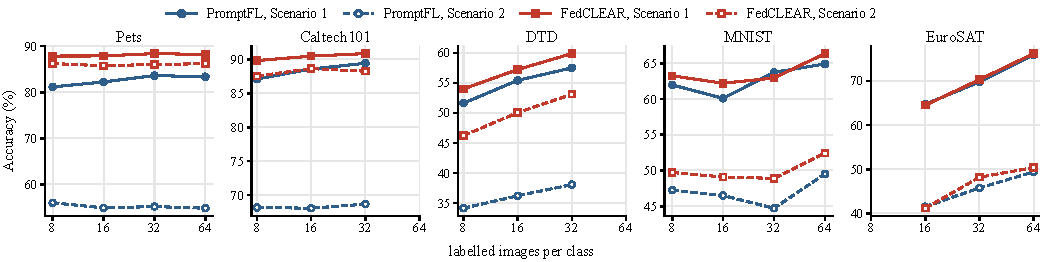
\includegraphics[width=\linewidth]{Figs/ShotStudy.pdf}
    \caption{Average accuracy (\%) of PromptFL and FedCLEAR over the settings of each scenario against
    the number of labelled images per class (mean of the last 10 rounds over 5 seeds). EuroSAT starts
    at 16 images because its 8-shot runs used the folder names of the classes instead of the CoOp class
    names; DTD has 60 training images per class, so its curves stop at 32.}
    \label{fig:shots}
\end{figure}

% \subsection{Client variation}
% em sẽ chạy hết dữ liệu với 10, 20, 50, 100 clients
% TODO (2026-11-16): no runs yet beyond the 10-client full-data batch; section left out until then.

\section{Conclusions}
\label{sec:concl}
We studied label noise in federated few-shot prompt learning and showed that a few noisy clients are
enough to make the learned prompt worse than zero-shot CLIP. FedCLEAR repairs the labels on each client
before local training, using a reference that averages the global prompt and zero-shot CLIP: the mean excess loss of the labels selects the clients to repair, suspect samples are relabelled when the reference is
confident and set aside otherwise, and under heavy noise a noise-aware temperature calibrates the
reference, a step enabled only when the clients' early reports show that the reference is reliable.
The method keeps
the communication of PromptFL. On five datasets and two noise scenarios it has the best or tied-best average
accuracy in nine of the ten combinations, with the largest gains when every client is noisy, and in
this scenario its lead over PromptFL persists with up to 32 or 64 labelled images per class on Pets,
Caltech101 and DTD; with five
seeds, however, most differences to the strongest baseline are within the seed-to-seed variation.
Its main limitation is its dependence on zero-shot CLIP: on domains far from natural images, such as
handwritten digits and satellite images, the reference is weak, the calibrated repair stays off and
the gains are smaller; with 75\% noise on MNIST, zero-shot CLIP remains more accurate than every
trained method. Our evaluation also has a limited scope: one backbone (CLIP with a ResNet-50 image
encoder), ten clients, 8 labelled images per class and five seeds. Other numbers of shots, larger and
more heterogeneous federations, other backbones, and stronger references for domains far from natural
images are left for future work.

% \appendix
% \section{Statistical comparison}
% \label{app:stats}
% Table~\ref{tab:app_mean} gives, for every method, the mean and standard deviation over the five seeds of
% the per-seed average over the settings of a scenario. Table~\ref{tab:app_test} compares FedCLEAR with
% each baseline by a paired $t$-test over the seeds; in every seed all methods see the same data, partition
% and wrong labels.
% \begin{table}[H]
% \centering
% \caption{Average accuracy (\%) over the settings of each scenario: mean $\pm$ standard deviation over the
% five seeds.}
% \label{tab:app_mean}
% \setlength{\tabcolsep}{3pt}
% \resizebox{\linewidth}{!}{%
% \begin{tabular}{llcccccc}
% \toprule[1.2pt]
% Scenario & Dataset & PromptFL & FedProx & FedCorr & NLPrompt & FedRG & FedCLEAR \\
% \midrule
% \multirow{5}{*}{1} & Pets       & 81.1$\pm$2.3 & 81.5$\pm$2.3 & 80.5$\pm$1.4 & 87.8$\pm$0.4 & 87.2$\pm$0.3 & 87.8$\pm$0.3 \\
%                    & Caltech101 & 87.1$\pm$0.5 & 87.3$\pm$0.6 & 88.3$\pm$0.9 & 89.5$\pm$0.6 & 89.7$\pm$0.5 & 89.8$\pm$0.5 \\
%                    & MNIST      & 62.0$\pm$2.9 & 62.4$\pm$2.6 & 59.9$\pm$2.8 & 54.4$\pm$5.5 & 58.2$\pm$4.3 & 63.2$\pm$2.6 \\
%                    & DTD        & 51.6$\pm$1.2 & 51.4$\pm$0.9 & 47.5$\pm$2.1 & 48.5$\pm$1.4 & 52.4$\pm$2.0 & 54.0$\pm$0.8 \\
%                    & EuroSAT    & 59.5$\pm$2.9 & 58.2$\pm$2.9 & 44.9$\pm$12.4 & 49.2$\pm$5.0 & 57.6$\pm$5.7 & 60.1$\pm$3.9 \\
% \midrule
% \multirow{5}{*}{2} & Pets       & 56.0$\pm$2.3 & 56.5$\pm$2.8 & 63.0$\pm$3.2 & 83.8$\pm$2.0 & 82.7$\pm$1.7 & 86.2$\pm$0.7 \\
%                    & Caltech101 & 68.2$\pm$2.6 & 67.4$\pm$3.0 & 73.5$\pm$2.8 & 87.1$\pm$1.4 & 87.8$\pm$0.7 & 87.5$\pm$1.5 \\
%                    & MNIST      & 47.3$\pm$2.3 & 47.3$\pm$2.3 & 43.2$\pm$6.4 & 41.2$\pm$5.7 & 42.7$\pm$1.6 & 49.7$\pm$5.4 \\
%                    & DTD        & 34.1$\pm$1.4 & 34.2$\pm$1.7 & 35.7$\pm$1.1 & 42.8$\pm$1.4 & 45.8$\pm$1.1 & 46.2$\pm$0.8 \\
%                    & EuroSAT    & 36.6$\pm$2.1 & 36.6$\pm$2.1 & 35.2$\pm$4.2 & 35.1$\pm$3.7 & 37.3$\pm$4.1 & 40.4$\pm$2.2 \\
% \bottomrule[1.2pt]
% \end{tabular}}
% \end{table}
% \begin{table}[H]
% \centering
% \caption{FedCLEAR minus each baseline on the averages of Table~\ref{tab:app_mean}: mean difference in points,
% $p$-value of the paired $t$-test over the five seeds, and number of seeds in which FedCLEAR is ahead.
% Differences with $p < 0.05$ are in bold.}
% \label{tab:app_test}
% \setlength{\tabcolsep}{3pt}
% \resizebox{\linewidth}{!}{%
% \begin{tabular}{llccccc}
% \toprule[1.2pt]
% Scenario & Dataset & vs.\ PromptFL & vs.\ FedProx & vs.\ FedCorr & vs.\ NLPrompt & vs.\ FedRG \\
% \midrule
% \multirow{5}{*}{1} & Pets       & \textbf{+6.7} (0.004, 5/5) & \textbf{+6.4} (0.004, 5/5) & \textbf{+7.4} (0.000, 5/5) & +0.0 (0.767, 2/5) & \textbf{+0.6} (0.037, 5/5) \\
%                    & Caltech101 & \textbf{+2.7} (0.001, 5/5) & \textbf{+2.5} (0.004, 5/5) & \textbf{+1.6} (0.048, 5/5) & +0.3 (0.376, 2/5) & +0.2 (0.424, 3/5) \\
%                    & MNIST      & +1.3 (0.340, 3/5) & +0.9 (0.264, 3/5) & \textbf{+3.4} (0.022, 5/5) & \textbf{+8.8} (0.007, 5/5) & \textbf{+5.0} (0.022, 5/5) \\
%                    & DTD        & \textbf{+2.4} (0.015, 5/5) & \textbf{+2.6} (0.014, 5/5) & \textbf{+6.5} (0.001, 5/5) & \textbf{+5.5} (0.000, 5/5) & +1.6 (0.105, 4/5) \\
%                    & EuroSAT    & +0.6 (0.636, 3/5) & +1.9 (0.260, 3/5) & \textbf{+15.2} (0.041, 5/5) & \textbf{+10.9} (0.000, 5/5) & +2.5 (0.205, 3/5) \\
% \midrule
% \multirow{5}{*}{2} & Pets       & \textbf{+30.2} (0.000, 5/5) & \textbf{+29.7} (0.000, 5/5) & \textbf{+23.2} (0.000, 5/5) & \textbf{+2.4} (0.024, 5/5) & \textbf{+3.5} (0.004, 5/5) \\
%                    & Caltech101 & \textbf{+19.4} (0.000, 5/5) & \textbf{+20.1} (0.000, 5/5) & \textbf{+14.0} (0.000, 5/5) & +0.4 (0.435, 2/5) & $-$0.3 (0.622, 1/5) \\
%                    & MNIST      & +2.5 (0.161, 3/5) & +2.5 (0.161, 3/5) & +6.5 (0.128, 4/5) & +8.6 (0.084, 4/5) & \textbf{+7.0} (0.036, 5/5) \\
%                    & DTD        & \textbf{+12.1} (0.000, 5/5) & \textbf{+12.0} (0.000, 5/5) & \textbf{+10.5} (0.000, 5/5) & \textbf{+3.5} (0.001, 5/5) & +0.4 (0.381, 4/5) \\
%                    & EuroSAT    & \textbf{+3.8} (0.038, 4/5) & \textbf{+3.8} (0.038, 4/5) & \textbf{+5.2} (0.030, 5/5) & \textbf{+5.3} (0.016, 5/5) & +3.2 (0.115, 4/5) \\
% \bottomrule[1.2pt]
% \end{tabular}}
% \end{table}

% \section{Zero-shot templates}
% \label{app:templates}

% \begin{table}[h]
% \centering
% \caption{Hand-crafted templates of zero-shot CLIP, used for the ZS-CLIP baseline, for the
% zero-shot term of the reference prediction (Eq.~\eqref{eq:ref}) and for the look-alike classes.
% [CLASS] is replaced by the class name.}
% \label{tab:templates}
% \begin{tabular}{lll}
% \toprule
% Dataset & Template & Source \\
% \midrule
% Oxford Pets & ``a type of pet, a photo of a [CLASS].'' & FLiP \cite{liao2025flip} \\
% Caltech101  & ``a photo of a [CLASS].''                & FLiP \cite{liao2025flip} \\
% DTD         & ``a texture of [CLASS].''                & FLiP \cite{liao2025flip} \\
% EuroSAT     & ``a centered satellite photo of [CLASS].'' & FLiP \cite{liao2025flip} \\
% MNIST       & ``a photo of the number: \textquotedbl[CLASS]\textquotedbl.''   & CLIP \cite{radford2021learning} \\
% \bottomrule
% \end{tabular}
% \end{table}

\bibliographystyle{splncs04}
\bibliography{PAKDD}

\end{document}
